\documentclass[12pt, a4paper]{article}
\usepackage{graphicx}
\usepackage{hyperref}
\usepackage[left=2cm, right=2cm, top=1cm]{geometry}
\title{Coursera Capstone Project - Week 4\\ \textbf{Finding US cities similar to Phoenix} }
\author{Bhaumik Choksi}

\begin{document}
	\maketitle
	
%\begin{figure}
%	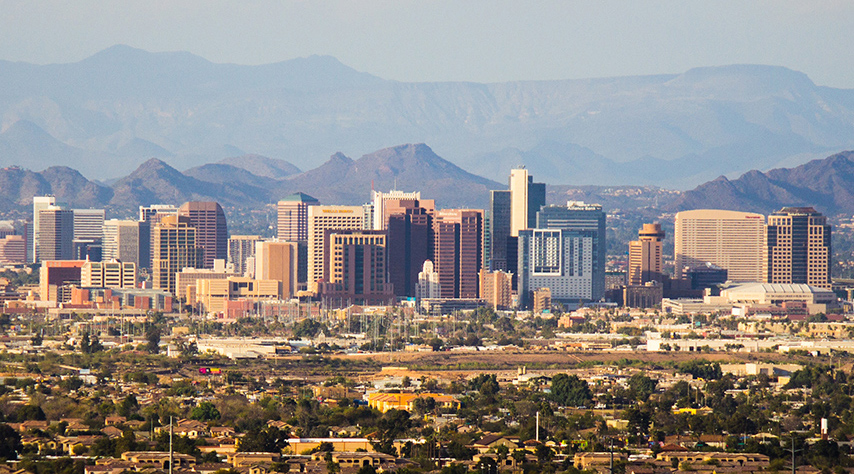
\includegraphics[width=200px]{phoenix}
%	\centering
%\end{figure}
	
%	\section*{Introduction}
%	A city can be defined broadly as a collection of various commercial, governmental and residential properties. Identifying similar cities can have many potential applications. Lawmakers, businesses and even common people can use these relationships to draw relevant insights. 
%	
%	This project aims to leverage location and venue data in order to identify cities similar to a given city (Phoenix, Arizona in this case). 
%	
%	
%	\section*{Business Problem}
%	Given a city, can we use the data about the nearby venues to identify other cities that are similar to the given city in terms of the composition and availability of these venues.
%	
%	More specifically, \textit{what cities in the US are similar to Phoenix in terms of venues}? 

\section*{Description of the data}
I will be using data from two different sources for this project - Foursquare and the US Cities Dataset. The Foursquare API provides data about the venues whereas the US Cities Dataset provides city names and location coordinates. 

\subsection*{Foursquare API}
Website: \href{https://developer.foursquare.com/docs/api/venues/details}{https://developer.foursquare.com/docs/api/venues/details}
\newline
The Foursquare Places API allows users to get details about nearby venues for a given location. I've used this API to get the following details about 10 nearby venues for a given city:
\begin{enumerate}
	\item Venue Name
	\item Venue Latitude
	\item Venue Longitude
	\item Venue Category (Short name)
\end{enumerate}

\subsection*{US Cities Dataset}
\begin{itemize}
	\item Original Name: 1000 Largest US Cities By Population With Geographic Coordinates
	\item Website: opendatasoft.com
	\item Source: \href{https://public.opendatasoft.com/explore/dataset/1000-largest-us-cities-by-population-with-geographic-coordinates/export/?sort=-rank&dataChart=eyJxdWVyaWVzIjpbeyJjb25maWciOnsiZGF0YXNldCI6IjEwMDAtbGFyZ2VzdC11cy1jaXRpZXMtYnktcG9wdWxhdGlvbi13aXRoLWdlb2dyYXBoaWMtY29vcmRpbmF0ZXMiLCJvcHRpb25zIjp7InNvcnQiOiItcmFuayJ9fSwiY2hhcnRzIjpbeyJhbGlnbk1vbnRoIjp0cnVlLCJ0eXBlIjoiY29sdW1uIiwiZnVuYyI6IkFWRyIsInlBeGlzIjoicmFuayIsInNjaWVudGlmaWNEaXNwbGF5Ijp0cnVlLCJjb2xvciI6IiNGRjUxNUEifV0sInhBeGlzIjoiY2l0eSIsIm1heHBvaW50cyI6NTAsInNvcnQiOiIifV0sInRpbWVzY2FsZSI6IiIsImRpc3BsYXlMZWdlbmQiOnRydWUsImFsaWduTW9udGgiOnRydWV9}{Click here}
	\item Reference: \href{https://gist.github.com/Miserlou/c5cd8364bf9b2420bb29#file-cities-json}{Miserlou on GitHub} 
	\item Disclaimer: I do not own any part of this dataset. All copyrights belong to their respective owners. 
\end{itemize}
I will be using the following columns from this dataset:
\begin{enumerate}
	\item City
	\item Rank
	\item Coordinates 
\end{enumerate}
	
\end{document}